\section{Bioetica 3: Comunicazione in medicina}

\subsection{Introduzione}

Il rischio clinico nasce dal fatto che manchi la comunicazione.
Comunicare è una delle cose più difficili in assoluto: spesso si
considera ovvio ciò che ovvio non è e non lo si comunica; non comunicare
l'ovvio significa commettere un errore e compiere un errore significa
far del male al paziente e a se stessi (come medici), questo soprattutto
alla luce del clima di tensione e contenzioso in cui si opera e in cui
l'opinione pubblica si orienta contro il medico (guarda il caso di
Saronno). Il rischio clinico è la professione, non è evitabile ma deve
essere combattuto per poterlo governare.

Seguono dei rudimenti sulla comunicazione essendo la comunicazione
importante per la professione.

Oggi comunicare è semplice, si comunica con i cellulari e questa è una
comunicazione sincopata, sintetica, essenziale ma a volte può portare a
fraintendimenti e incomprensioni e la capacità di comunicare in questo
modo dipende da una serie di fattori quali la cultura, la formazione,
l'età. Ma la comunicazione deve essere multipla e a multipli livelli e
tutti devono essere in grado di comunicare.

Principi della comunicazione nella professione medica (Sottosezione)

\subsubsection{Codice deontologico}

La professione è regolamentata da una serie di principi, in primis dal
codice deontologico che consiste in un insieme di regole che
disciplinano il comportamento del medico; seguire tali regole permette
di evitare errori e comportamenti che possano compromettere la
professione e il rapporto medico paziente.

Il rapporto medico paziente è alla base della professione: è un rapporto
esclusivo e di interdipendenza in cui il medico è il punto di
riferimento per la salute del paziente. Gli articoli del codice
deontologico che si riferiscono al rapporto medico paziente sono i
seguenti: art. 20, 33, 34, 37. Di seguito non sono riportati gli
articoli (per questi vedere le slide) ma il commento del prof a tali
articoli.

\begin{itemize}
\item
  art. 33 ovvero comunicazione e informazione con la persona assistita
  (2014): si considera il paziente come persona che sta male e non come
  malattia.
\item
  art 34 ovvero informazione e comunicazione
\item
  art. 37 ovvero consenso e dissenso informato: consenso informato
  significa che il medico è autorizzato a fare qualsiasi cosa per la
  quale il paziente abbia dato il proprio consenso, dissenso significa
  che il paziente in qualunque momento può dissentire e non consentire a
  quanto precedentemente concordato, il medico quindi non è autorizzato
  a proseguire con il percorso intrapreso, in ultima istanza il paziente
  può accettare ma allo stesso tempo recedere da qualsiasi percorso
  diagnostico terapeutico proposto dal medico.
\item
  art. 20 ovvero relazione di cura: recente, il tempo della
  comunicazione non è tempo perso ma è considerato tempo di cura, grande
  importanza hanno l'ascolto e la comunicazione.
\end{itemize}

\begin{itemize}
\item
  Il primo presupposto di una buona relazione medico paziente è
  l'uguaglianza tra le parti: uguaglianza intesa non in senso
  democratico ma nel senso di riconoscere le differenze culturali e di
  adattarsi a queste: se il paziente non è in grado di comprendere il
  linguaggio scientifico e la terminologia appropriata, allora il medico
  deve parlare in modo che venga capito, deve abbassare il proprio
  linguaggio, parlare in modo quanto più semplice è possibile.
\item
  Il secondo presupposto è il riconoscimento reciproco ovvero
  riconoscere il valore del proprio interlocutore e non essere quindi
  superficiali nel comportamento.
\item
  Il terzo presupposto è la necessità di rispetto e considerazione.
  Esempio: quando qualcuno parla, la considerazione che chi ha ascolta
  ha di lui si vede negli atteggiamenti. Anche il medico valutando il
  paziente capisce che considerazione il paziente ha di lui, riuscendo
  ad esempio ad individuare quei pazienti che hanno scarsa
  considerazione del medico perché sono convinti di aver già fatto
  diagnosi del proprio disturbo consultando Internet.
\end{itemize}

Osservando il paziente il medico può adattare il proprio comportamento
così che la relazione di cura sia efficace. Il medico ricorre all'arte
suasoria per convincere il malato ad eseguire le procedure diagnostiche
e terapeutiche che sono opportune. Esempio: convincere un paziente
ansioso -- depresso ad assumere un ansiolitico -- antidepressivo
potrebbe non essere semplice perché il paziente crede che il medico lo
creda pazzo ma il medico, se è convinto che la terapia sia opportuna
perché si tratta di sintomi sovra strutturati, non associati a nulla di
organico, deve convincere il paziente ad assumere i farmaci.

Comunicare non significa solo informare ma significa far capire. La
comunicazione in medicina è importante perché le incomprensioni --fino
al contenzioso­­-- tra medico e paziente nascono perché la comunicazione
non è stata efficace. La comunicazione inoltre ha i suoi tempi e questi
devono essere rispettati: i medici vengono segnalati all'ordine dei
medici per la frettolosità con cui comunicano con il paziente perché
questo è un aspetto molto sentito dal paziente.

\subsection{Watzlawick}

\subsubsection{Definizione di comunicazione}

Secondo Paul Watzlawick la comunicazione è uno scambio imperativo tra
due o più partecipanti dotato di intenzionalità reciproca e di un certo
livello di consapevolezza, in grado di far condividere un determinato
significato sulla base di sistemi simbolici e convenzionali di
significazione e di segnalazione secondo la cultura di
riferimento\emph{.}

Considerazione che scaturisce da questa definizione: un medico che
utilizza termini scientificamente validi ma dotti, che il malato non
conosce, non è un medico che opera per il bene del paziente perché non
comunica, per comunicare bisogna farsi capire e il linguaggio
scientifico impedisce l'interazione con il paziente (è come parlare allo
specchio), crea una frattura. Ricordate il malato immaginario di
Molière. Quindi il tempo della comunicazione è un tempo di cura, una
buona comunicazione rafforza l'alleanza medico paziente.

\subsubsection{Gli assiomi della comunicazione}

\begin{itemize}
\item[1.]
  \emph{È impossibile non comunicare}
\item[2.]
  \emph{Livelli comunicativi di contenuto e relazione: ad ogni
  comunicazione si associa una meta comunicazione.}
\item[3.]
  \emph{Punteggiatura della sequenza di eventi: la natura di una
  relazione dipende anche dalla punteggiatura delle sequenze di scambi
  comunica-tivi tra i comunicanti.}
\item[4.]
  \emph{Comunicazione numerica e analogica: gli esseri umani hanno la
  capacità di comunicare sia tramite un modulo comunicativo digitale (o
  numerico) sia con un modulo analogico.}
\item[5.]
  \emph{Interazione complementare e simmetrica: classificazione della
  natura delle relazioni che le suddivide in relazioni basate
  sull'uguaglianza oppure sulla differenza. Nel primo caso si parla di
  relazioni simmetriche, in cui entrambi i partecipanti tendono a
  rispecchiare il comportamento dell'altro (ad es. nel caso della diade
  dirigente-dirigente, o dipendente-dipendente); nel secondo si parla di
  relazioni complementari, in cui il comportamento di uno dei
  comunicanti completa quello dell'altro (ad es. dirigente-dipendente).}
\end{itemize}

\subsection{Comunicatori si nasce o si diventa?}

Entrambe: ci sono medici che nascono come comunicatori, che sono
empatici (l'empatia non è farsi carico dei problemi dell'altro ma è
essere di supporto) e ci sono medici che non sono comunicatori (``è un
bravissimo medico ma è freddo come il ghiaccio'').

Un soggetto può essere inconsapevole -- consapevole di non saper
comunicare e consapevole -- inconsapevole di saper comunicare. Nel
dettaglio, in sequenza:

\begin{itemize}
\item[1.]
  essere inconsapevoli di non saper comunicare, non si ha la
  consapevolezza della propria mancanza;
\item[2.]
  essere consapevoli di non saper comunicare, si ha la consapevolezza
  della propria mancanza e ci si applica per migliorare;
\item[3.]
  essere consapevoli di saper comunicare, la capacità di comunicare si
  accresce;
\item[4.]
  essere inconsapevoli di saper comunicare, la comunicazione è spontanea
  e naturale.
\end{itemize}

\subsection{Elementi della comunicazione}

La comunicazione è il processo con cui messaggi opportunamente
codificati vengono scambiati tra emittente e ricevente. Emittente è
colui che dà il messaggio, ricevente è colui che riceve il messaggio. La
relazione tra emittente e ricevente si instaura quando il contenuto del
messaggio viene condiviso.

\subsubsection{Trasmissione e diario clinico}

La trasmissione consiste nella progressione del messaggio. Deve essere
corredata e correlata da un sistema di diffusione che sia oggettivo,
dimensionato e orientato altrimenti si rischia che ci si siano
fraintendimenti. Esemplificativo del rischio di fraintendimento
associato alla trasmissione di un messaggio è il gioco per bambini ``il
telefono senza fili''. Esempio: al cambio guardia un medico riferisce al
collega che subentra la terapia somministrata al paziente, ma si
scambiano una parola al volo, chi subentra non capisce se sia stata
somministrata vit. B o digitale. Da ciò scaturisce la necessità del
diario clinico.

Il diario clinico ha tre significati: professionale, deontologico,
giuridico.

\begin{itemize}
\item
  significato professionale: il medico è tenuto a registrare ogni atto
  compiuto sul paziente. Esempio: ore x crisi asmatica, esame obiettivo,
  trattamento eseguito; ore x + y rivalutazione, evoluzione positiva/
  negativa, supplemento diagnostico e/o terapeutico.
\end{itemize}

Così i colleghi possono sapere cos'è successo e cosa è stato fatto.

\begin{itemize}
\item
  significato deontologico: ogni atto eseguito sul paziente deve essere
  attestato.
\item
  significato giuridico: è dovere del medico attestare tutto quello che
  è stato fatto; addirittura buona parte delle condanne penali sono
  dovute al fatto che non sia stato compilato il diario clinico. Anche
  il medico di famiglia scrive il diario clinico, non perché abbia
  l'obbligo di farlo ma perché nel farlo si tutela. Il medico si spera
  che operi in scienza e coscienza ma se fosse citato in giudizio può
  presentare il diario clinico (scritto, non modificabile) come prova a
  proprio favore.
\end{itemize}

Ovviamente nel diario clinico bisogna riportare il vero, non si può
attestare il falso.

\subsection{Jakobson e le sei funzioni della comunicazione}

Gli aspetti fondamentali della comunicazione sono: il mittente, il
messaggio che deve avere un significato, il destinatario, il contesto,
il codice (linguaggio comune a mittente e ricevente) e un canale (mezzo)
di comunicazione per passare il messaggio.

Come valutare l'efficacia della comunicazione. Con il feed back. Il feed
back è rappresentato dagli atteggiamenti (toccarsi, grattarsi) e dalle
espressioni del volto di chi ascolta, si tratti di segnali non verbali.
Grazie al feed back il medico adatta il proprio modo di comunicare per
far si che il ricevente riceva effettivamente il messaggio.

\subsection{Linguaggi non verbali}

I linguaggi non verbali integrano il linguaggio verbale: alle parole
seguono i gesti. Il gesticolare può accrescere il significato di un
termine, può racchiudere in se un termine, può incentivare
l'interlocutore a partecipare o allontanarlo.

\subsubsection{Postura} 

Il linguaggio di relazione è la postura, è il modo con cui ci
atteggiamo, è il modo con cui ci avviciniamo all'altro.
Dall'atteggiamento e della postura si stabilisce la natura della
relazione tra due interlocutori, se intima, professionale, pubblica. In
una relazione intima come in un rapporto di amicizia non ci sono
barriere, in una relazione professionale le distanze aumentano, in una
relazione pubblica aumentano ulteriormente.

L'atteggiamento di chi ascolta un messaggio può essere di apertura, di
chiusura, di sfida. Esempio: raccogliendo un'anamnesi è possibile che il
paziente assuma un atteggiamento difensivo (braccia conserte), questo
perché ha paura. Esempio: quando il proprio interlocutore non presta
attenzione a ciò che si dice, parla al cellulare, controlla i messaggi
al cellulare, guarda dappertutto anziché fissare lo sguardo allora non è
interessato; non è detto che la responsabilità sia di chi ascolta,
potrebbe essere anche di chi parla. Nel caso del rapporto medico
paziente la responsabilità è del medico perché il medico è in una
posizione di potere dal momento che è lui che comunica la buona o la
cattiva notizia.

\subsubsection{Mimica}

La mimica facciale è espressione di quello che il paziente sente e
prova: sorpresa, paura, collera, disgusto, tristezza, felicità.

\subsubsection{Abbigliamento}

L'abbigliamento è significativo di un'impostazione mentale, l'assenza di
cravatta, i pantaloncini corti hanno il loro significato. Ciò che conta
è che il medico si presenti come una persona ben messa e pulita, un
medico pulito è sempre ben accetto dal paziente che è sempre molto
attento a questo.

\subsubsection{Prossemica}

La prossemica è la distanza interpersonale nei rapporti.

\begin{itemize}
\item
  \textless{} 30 cm: zona intima
\item
  30 cm -- 1 m: zona personale
\item
  1 -- 3 m: zona sociale (esempio: distanza tra relatore e uditorio ad
  un convegno)
\item
  \textgreater{} 3 m: zona pubblica.
\end{itemize}

Rientra nella prossemica il problema del tocco: tra amici (zona intima)
è normale il tocco (mano sulla spalla). Esempio: gli anziani cercano il
contatto umano e durante la visita toccano la mano del medico e il
medico che si ritira dal tocco ritrae una parte di sé. Essere
fisicamente vicino al paziente abbatte le barriere.

La distanza interpersonale e il contatto possono essere interpretati in
maniera diversa a seconda delle abitudini di un popolo: i popoli nordici
- anglosassoni non gradiscono il contatto fisico (esempio l'abbraccio
tra sconosciuti) e un gesto di fraternità potrebbe essere frainteso.

\subsubsection{Linguaggio degli oggetti}

Frapporre una scrivania tra medico e paziente mette distanza, tutela
quel timore reverenziale necessario perché non si verifichi l'inversione
del rapporto medico paziente.

\subsubsection{Linguaggio paraverbale}

Per linguaggio paraverbale si intende il tono della voce: urlare,
parlare, sussurrare. Condiziona in maniera significativa il rapporto
comunicativo.

\subsubsection{Linguaggio del corpo}

\begin{itemize}
\item
  assertivo: espressione del volto interessata, occhi contatto oculare
  diretto, voce chiara, mani che non superano l'altezza dei gomiti;
\item
  aggressivo: espressione del volto tesa, non sorridente, occhi vitrei,
  voce alta, gestualità intimidatoria;
\item
  passivo: accondiscendenza, sorriso di convenienza, testa china, voce
  bassa, gestualità tesa.
\end{itemize}

\begin{itemize}
\item
  Pensare = 100\%
\item
  Dire = 70\%
\item
  Ricevere = 40 \%
\item
  Capire = 20\%
\item
  Ricordare = 10\%
\end{itemize}

\subsection{Quadrato della comunicazione di Von Thun}

Esistono 4 orecchie che ascoltano: orecchio giallo, blu, verde e rosso.
Queste servono per creare una relazione tra due soggetti. Fondamentale
è: 1) avere considerazione di se e 2) legittimare l'interlocutore,
significa considerarlo e metterlo nella condizione di farlo partecipe
della comunicazione e 3) la visione della realtà: dobbiamo utilizzare
tutti gli strumenti perché dalla realtà fattuale ci sia la giusta
acquisizione della realtà soggettiva che è la realtà interpretata.

 \begin{figure}[!ht]
\centering
	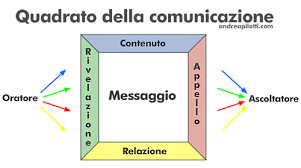
\includegraphics[width=0.5\textwidth]{31/image1.png}
	\end{figure}

 \begin{figure}[!ht]
\centering
	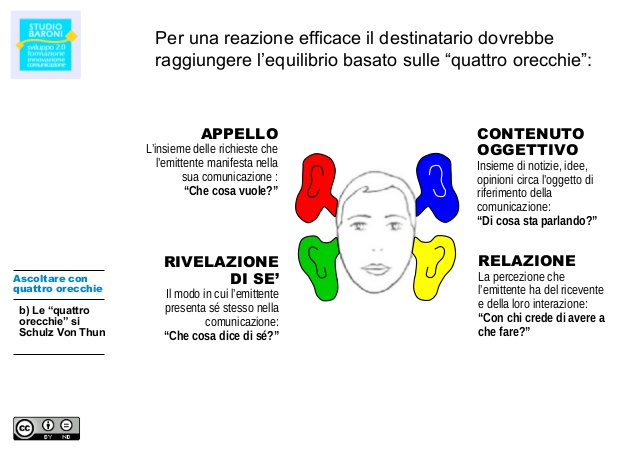
\includegraphics[width=0.5\textwidth]{31/image2.jpeg}
	\end{figure}

\subsection{Empatia e ascolto}

Empatia significa comprensione della situazione delx paziente, dei
sentimenti, delle emozioni e delle aspettative. Esempio: ``Dottore avrò
da star male? Mi aspetta qualcosa di brutto? Quanto tempo ho da
vivere?''. L'empatia è bloccata dal senso di superiorità, ecco perché è
necessario invece il rispetto: il medico deve rispettare il paziente e
allo stesso tempo il paziente deve rispettare il medico, i ruoli non si
devono invertire. L'empatia è facilitata dalla capacità di mimetismo del
medico, è la stessa capacità di un venditore che capisce cosa vuole il
cliente e riesce a vendere: il medico capisce il paziente, modifica
grazie al feed back paziente il proprio comportamento e si atteggia in
modo tale da far compiere al paziente le procedure che ritiene
opportune. Per il mimetismo è importante ascoltare. Dice Plutarco (35
d.C.): ``noi abbiamo due orecchie e una sola lingua perché siamo tenuti
ad ascoltare''.

L'ascolto attivo articola così:

\begin{itemize}
\item[1.]
  ascoltare e capire
\item[2.]
  valutare e controllare la comunicazione
\item[3.]
  dare delle risposte, essere un buon emittente.
\end{itemize}

Importante che ci sia compartecipazione, chiarezza, conoscenza e scelta
di metodo. I killer della comunicazione sono gli atteggiamenti e i
discorsi ambigui, le allusioni.

La gran parte di quello che i medici sanno la sanno grazie ai pazienti,
comunicare con gli ammalati significa imparare a fare i medici.